\documentclass{article}

\usepackage{algorithmicx}
\usepackage{algpseudocode}
\usepackage{graphicx}
\usepackage{listings}
\usepackage{amsmath}
\usepackage{textcomp}
\usepackage{color}
\usepackage[%  
    colorlinks=true,
    pdfborder={0 0 0},
    linkcolor=blue
]{hyperref}

\lstset{ %
  language=Java,                  % the language of the code
  basicstyle=\footnotesize,       % the size of the fonts that are used for the code
  numbers=left,                   % where to put the line-numbers
  numberstyle=\tiny\color{gray},  % the style that is used for the line-numbers
  stepnumber=1,                   % the step between two line-numbers. If it's 1, each line
                                  % will be numbered
  numbersep=5pt,                  % how far the line-numbers are from the code
  backgroundcolor=\color{white},  % choose the background color. You must add \usepackage{color}
  showspaces=false,               % show spaces adding particular underscores
  showstringspaces=false,         % underline spaces within strings
  showtabs=false,                 % show tabs within strings adding particular underscores
  frame=single,                   % adds a frame around the code
  rulecolor=\color{black},        % if not set, the frame-color may be changed on line-breaks within not-black text (e.g. commens (green here))
  tabsize=4,                      % sets default tabsize to 2 spaces
  captionpos=b,                   % sets the caption-position to bottom
  breaklines=true,                % sets automatic line breaking
  breakatwhitespace=false,        % sets if automatic breaks should only happen at whitespace
  title=\lstname,                 % show the filename of files included with \lstinputlisting;
                                  % also try caption instead of title
  keywordstyle=\color{blue},          % keyword style
  commentstyle=\color{dkgreen},       % comment style
  stringstyle=\color{mauve},         % string literal style
  escapeinside={\%*}{*)},            % if you want to add a comment within your code
  morekeywords={*,...}               % if you want to add more keywords to the set
}

\newcommand{\comment}[1]{}

\title{Assignment Week 4 - Questions and Solutions}
\author{Course: Building Blocks of Programming}
\date{Topic: Flowcharts - Arrays}
\begin{document}
\maketitle

\begin{flushleft}

    \textbf{Q 1. } Draw a flowchart that takes as input an integer N, 
    the size of an array, and then N integer elements of an array and print “yes” 
    if the array is a palindrome, otherwise print “no”
    
    \end{flushleft}
    
    \begin{flushleft}
    
    \textbf{Ans. } We can check for each valid index $i$ (for 0 based arrays this is 
    from 0 to $N-1$), whether $i^{th}$ and $(n-i-1)^{th}$ index are same or not. If and only 
    if the condition is satisfied for all indices, the array is a palindrome. The flowchart is in 
    Fig. \ref{Q1}
    
    \end{flushleft}
    
    \begin{flushleft}
    
    \textbf{Grading. } If the flowchart is correct then 2, if there are any errors in the flowchart but 
    the logic is correct then 1, otherwise 0. 
    
    \end{flushleft}
    
    \begin{figure}[ht]
        \centering
        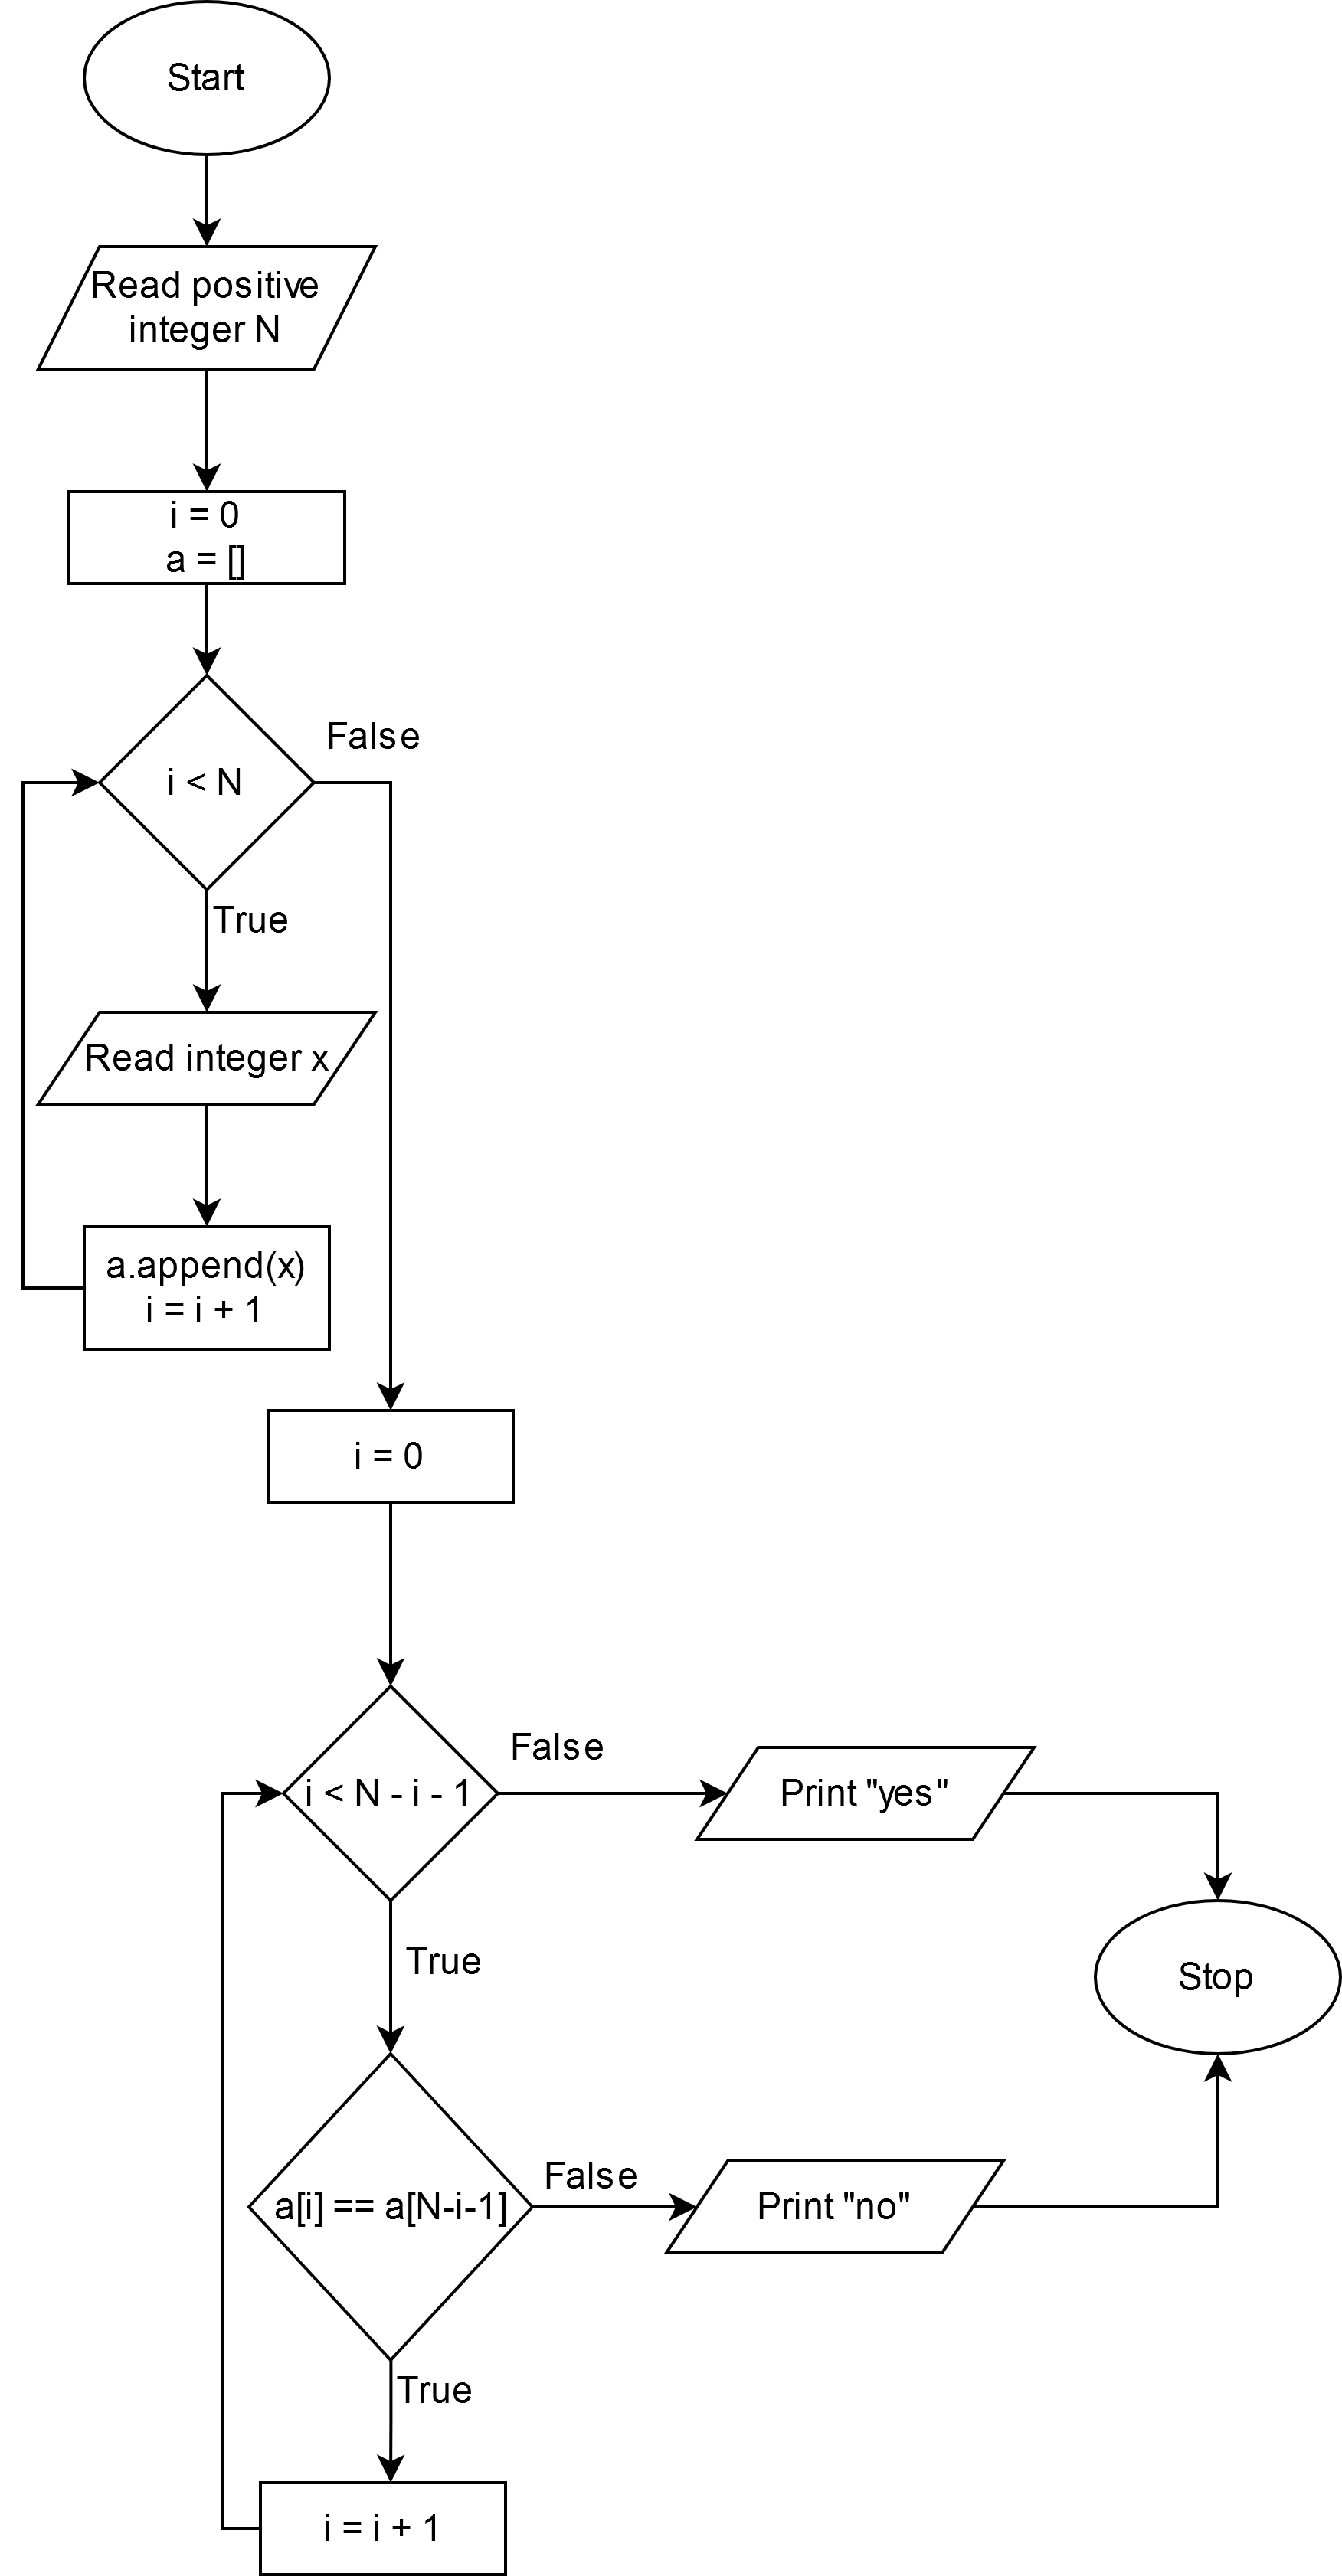
\includegraphics[width=0.5\textwidth]{Q1.png}
        \caption{Sample flowchart for Q1}
        \label{Q1}
    \end{figure}
\clearpage


\begin{flushleft}

\textbf{Q 2. } Draw a flowchart that takes integers as input, until the value “0” is given, and prints all 
the integers that were given before “0” in reverse order.

For example for the input,
    1 2 3 4 9 0
The output should be 
    9 4 3 2 1
\end{flushleft}

\begin{flushleft}

\textbf{Ans. } We should use an array to store the values so that we can revisit them in the reverse order 
and print them. The flowchart is in Fig \ref{Q2}.

\end{flushleft}

\begin{flushleft}

\textbf{Grading. } If the output is correct then 2, if there are any errors in the flowchart then 1,
otherwise 0.

\end{flushleft}

\begin{figure}[ht]
    \centering
    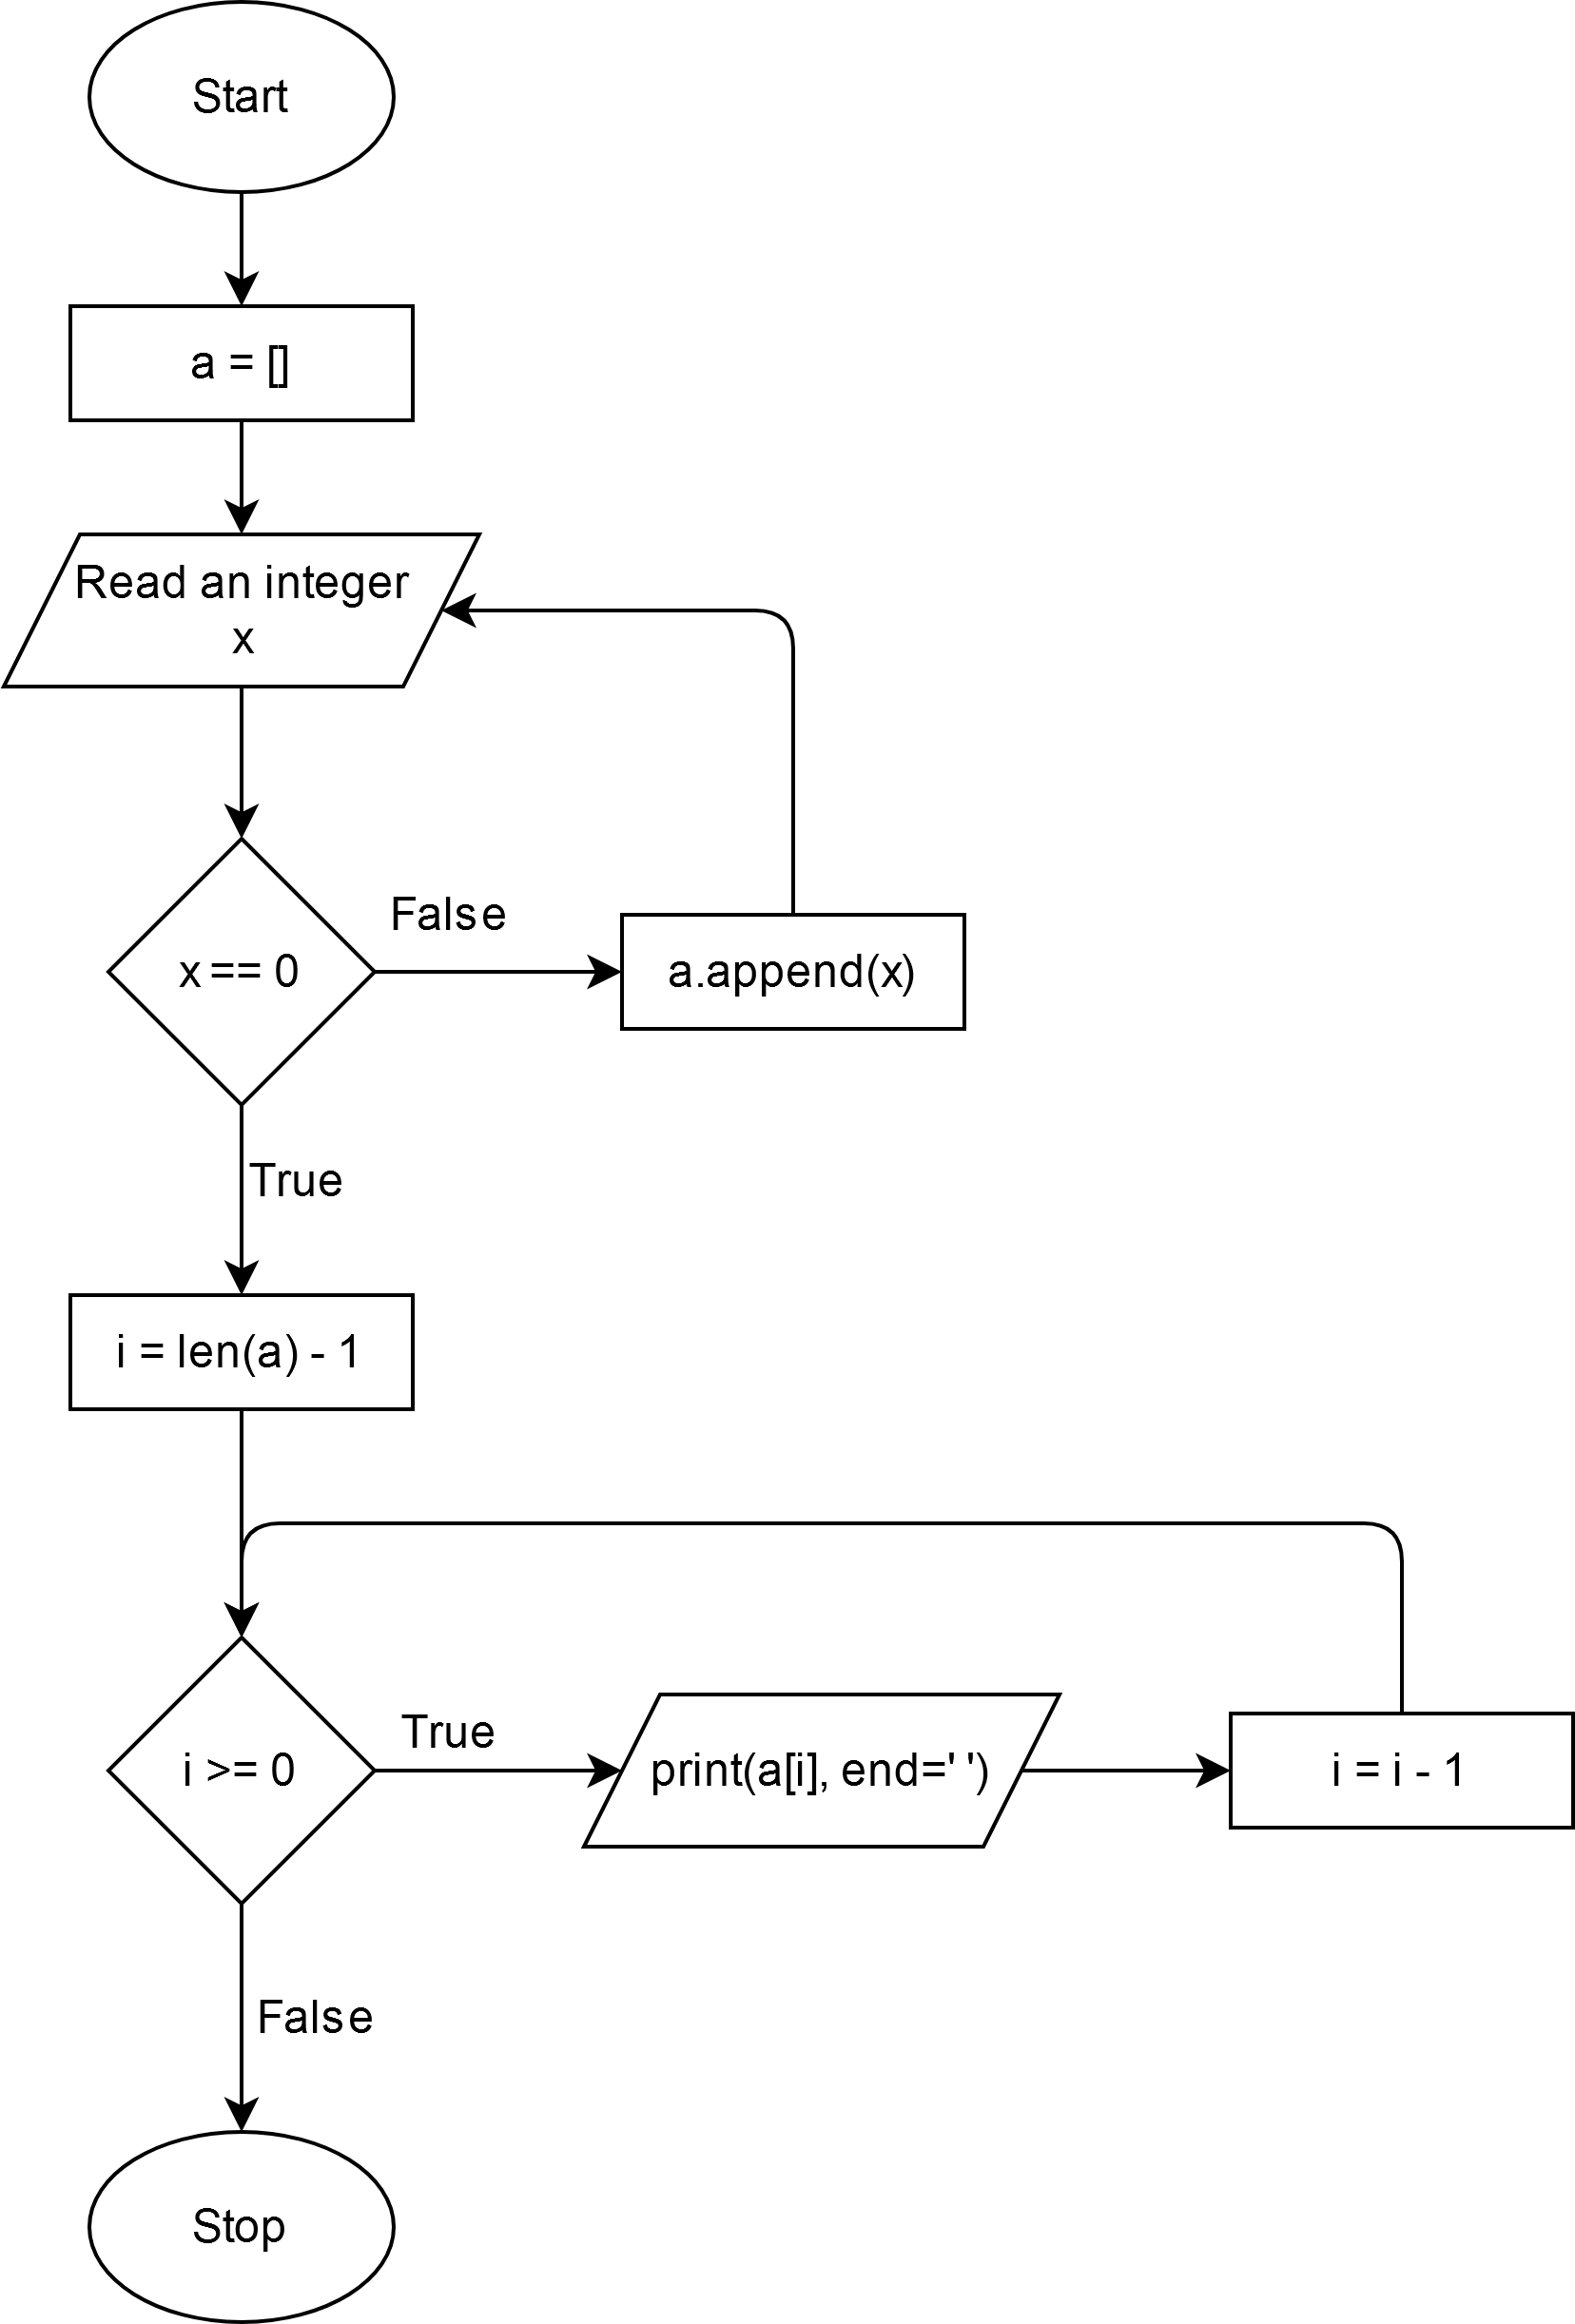
\includegraphics[width=0.5\textwidth]{Q2.png}
    \caption{Sample flowchart for Q2}
    \label{Q2}
\end{figure}

\clearpage


\begin{flushleft}

    \textbf{Q 3. } Draw a flowchart that takes as input an array of size N
    and prints the number of occurrences of the maximum value in the array. 
    Specifically, the inputs should be
    \begin{enumerate}
    \item  a positive integer N
    \item  N integers denoting the elements of the array
    \end{enumerate}
and the output should be an integer that denotes the number of occurrences of the maximum value in the array.
For example for the input,
   6
   3 1 3 3 2 3
the output should be,
   4
because there are 4 values equal to 3.
    
    \end{flushleft}
    
    \begin{flushleft}
    
    \textbf{Ans. } An easy solution is to store all the elements in an array, 
    find the maximum value and traverse the array a second time and find the 
    count of the maximum value. This is shown in Fig \ref{Q3}.
    We can also solve this problem by just reading the elements and maintaining the 
    maximum value of elements read so far and their count. We will update the maximum 
    value if the next element is strictly greater than the current maximum and reset count to 1.
    If the next element is equal to the current maximum then increase count by 1.
    This optimisation is not required.
    
    \end{flushleft}
    
    \begin{flushleft}
    
    \textbf{Grading. } Any solution that prints the correct output for all valid inputs give 2, if there 
    are any mistakes in the flowchart then 1, otherwise 0.
    
    \end{flushleft}
    
    \begin{figure}[ht]
        \centering
        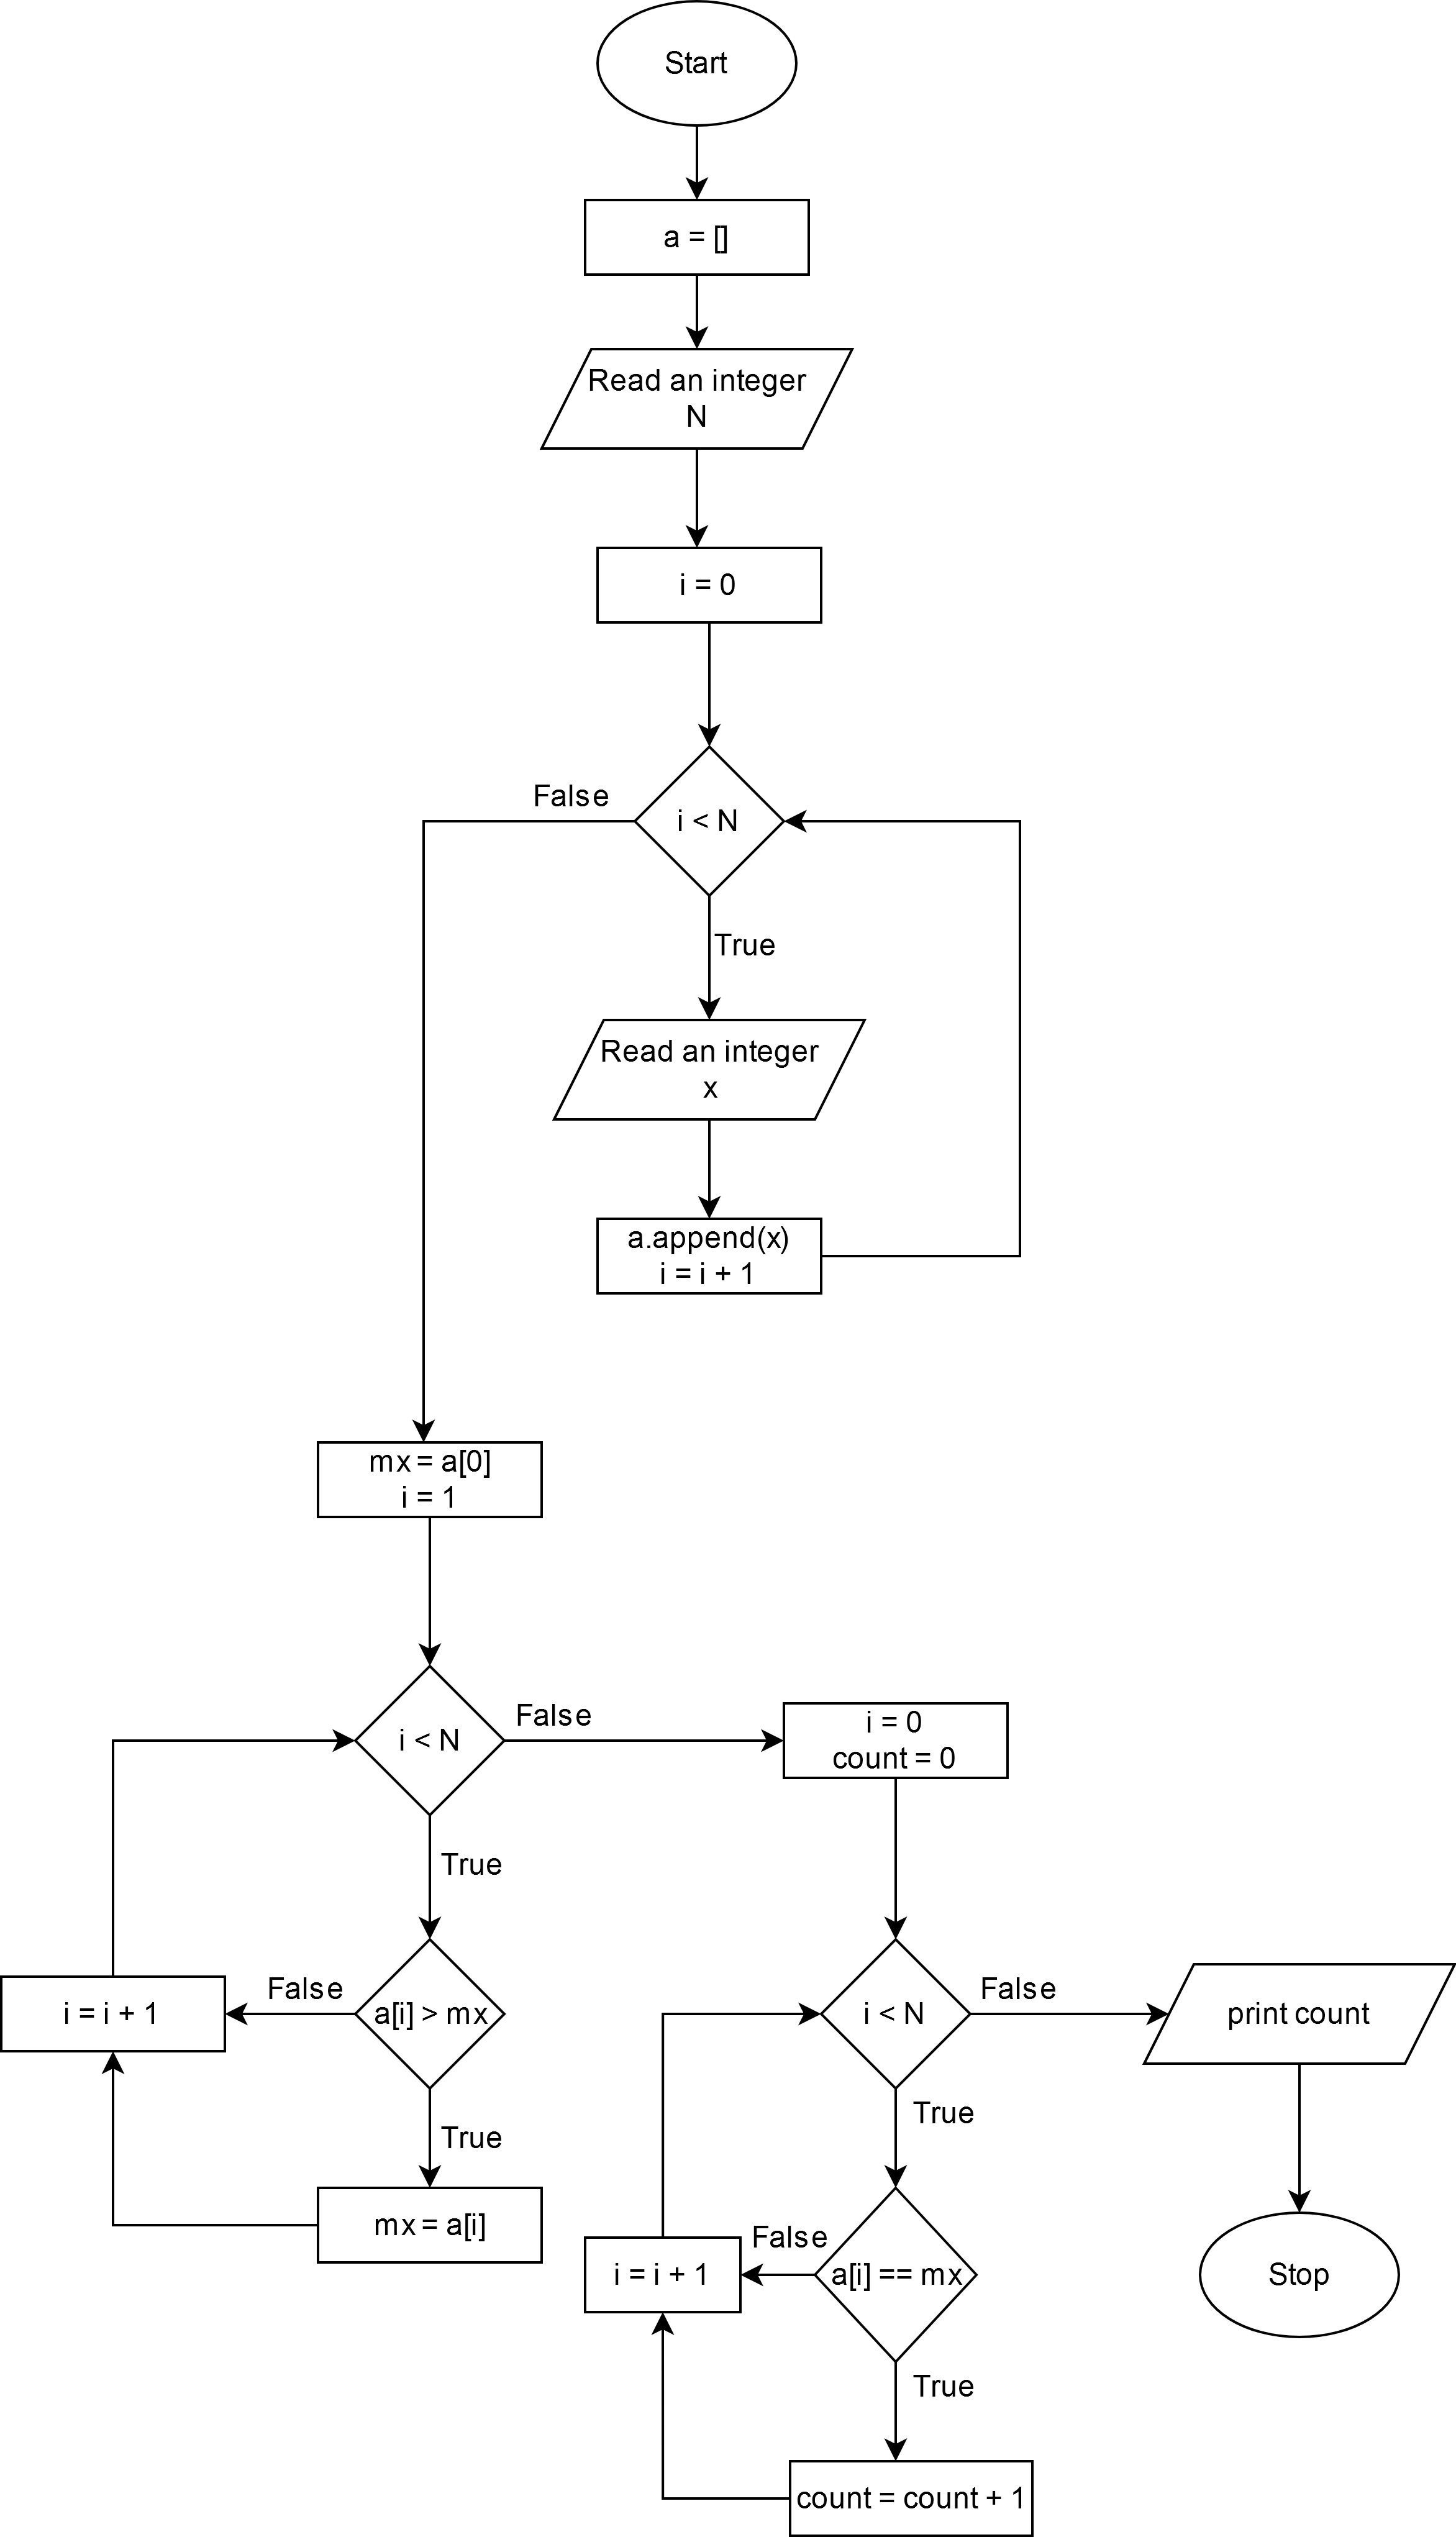
\includegraphics[width=0.5\textwidth]{Q3.png}
        \caption{Sample flowchart for Q3}
        \label{Q3}
    \end{figure}
    
    \clearpage


    \begin{flushleft}

        \textbf{Q 4. } Draw a flowchart that takes as input
        \begin{enumerate}
            \item a positive integer N
            \item N integers
        \end{enumerate}
    and prints all the numbers in even position (numbered from 1) first, followed by all the numbers in an odd position.
    For example for the input,
        5
    2 3 4 2 3 
    The output should be,
        3 2 2 4 3
    The numbers at even positions are “3, 2” and those at odd positions are “2, 4, 3”
    
        
        \end{flushleft}
        
        \begin{flushleft}
        
        \textbf{Ans. } We need to store all the inputs in an array so that we can traverse them in the 
        given order. We iterate through the array twice, in the first time we print only those values such 
        that the 0-based index is odd, in the second time we print only those values which are even.
        This is shown in Fig \ref{Q4}
        
        \end{flushleft}
        
        \begin{flushleft}
        
        \textbf{Grading. } Any flowchart that prints the correct output given the input give 2, if there 
        are any errors in the flowchart but the logic is correctly identified then 1, otherwise 0.
        
        \end{flushleft}
        
        \begin{figure}[ht]
            \centering
            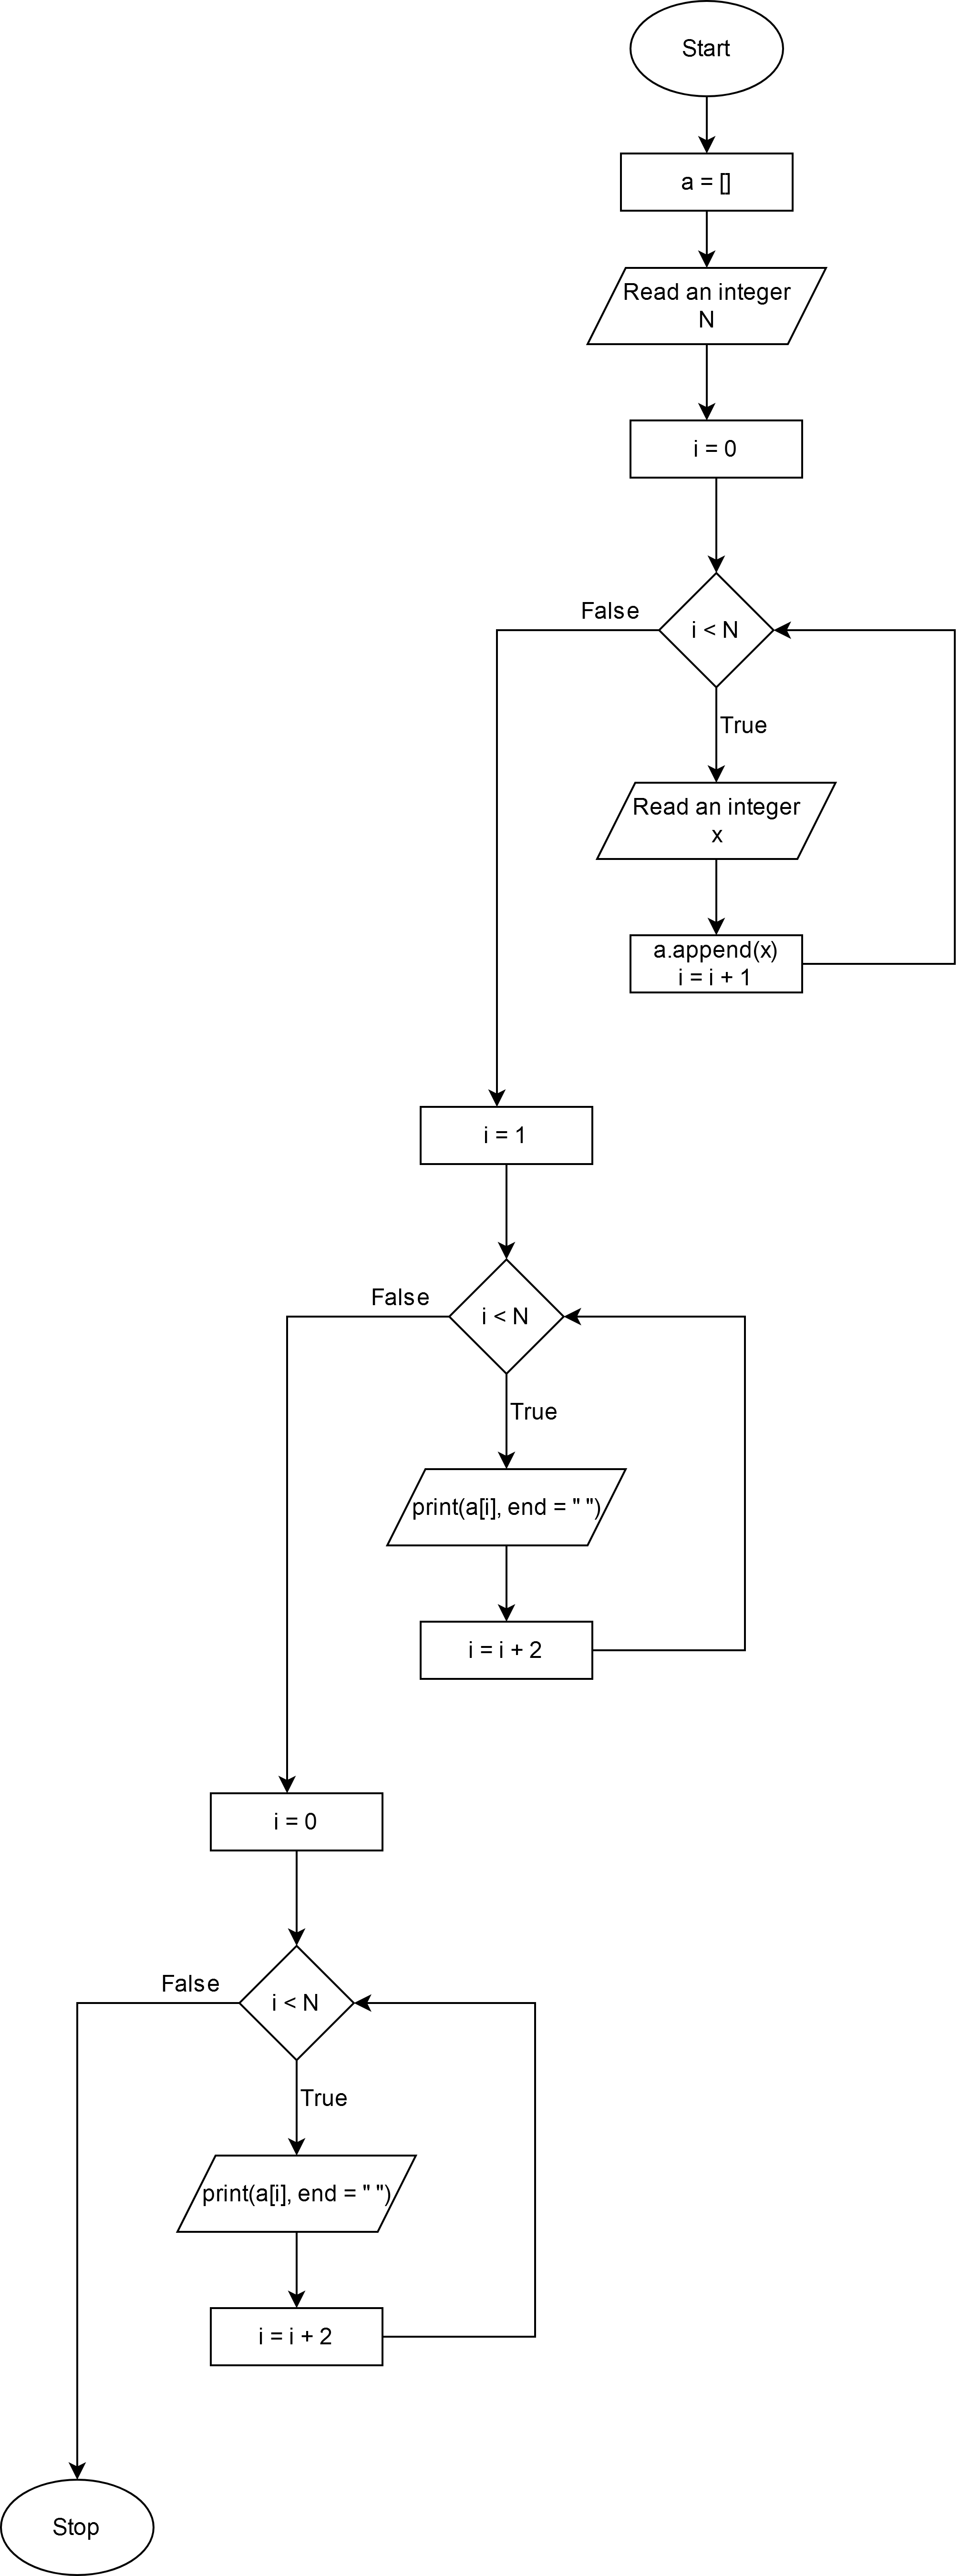
\includegraphics[width=0.5\textwidth]{Q4.png}
            \caption{Sample flowchart for Q4}
            \label{Q4}
        \end{figure}
        
        \clearpage


\begin{flushleft}

\textbf{Q 5. } Draw a flowchart that takes as input 
\begin{enumerate}
    \item an integer N
    \item N integers denoting an array A
    \item N integers denoting an array B
\end{enumerate}
and prints N integers, denoting an array C, which is obtained by adding the corresponding elements of A and B. 
For example for the sample input,
    2
    1 3
    4 5
the output should be 
    5 8


\end{flushleft}

\begin{flushleft}

\textbf{Ans. } We can simple read the arrays A, B and print their sum. This is shown in Fig \ref{Q5}.
We need not explicitly construct the array C, since only the output is required, however it is not wrong
to do so.

\end{flushleft}

\begin{flushleft}

\textbf{Grading. } Any flowchart that prints the given output for all valid inputs is given 2. Solutions that 
don't explicitly store the array B and just print after reading them is also correct. It is also allowed 
to explicitly construct the array C, and use "print C" in the flowchart.
Any errors in the flowchart results in 1, if there are any errors in the logic then 0.

\end{flushleft}

\begin{figure}[ht]
    \centering
    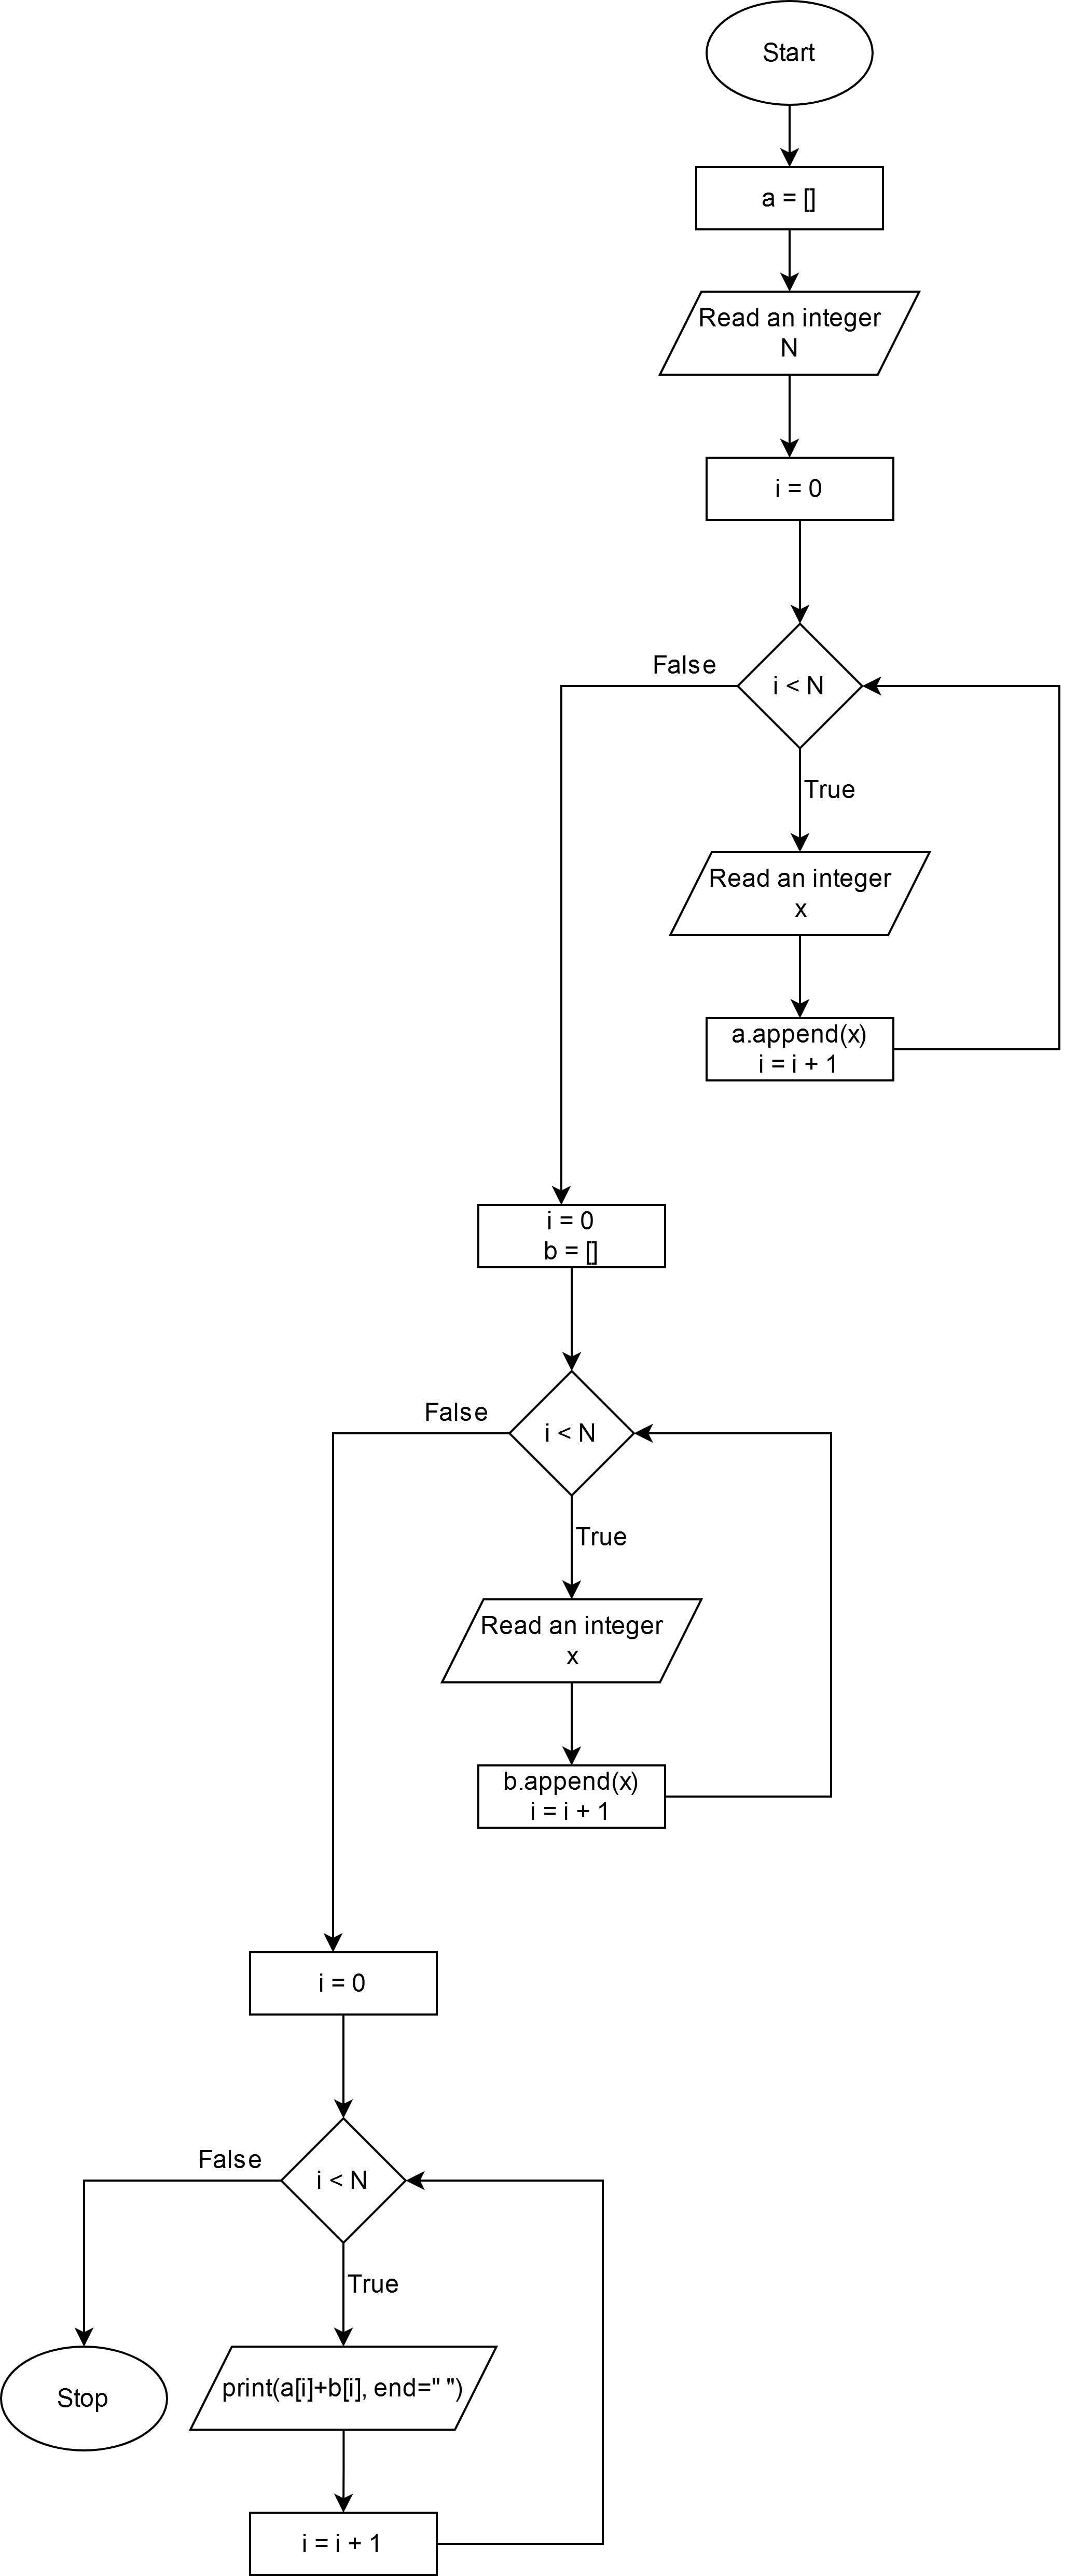
\includegraphics[width=0.5\textwidth]{Q5.png}
    \caption{Sample flowchart for Q5}
    \label{Q5}
\end{figure}

\clearpage


\begin{flushleft}

\textbf{Q 6. } Draw a flowchart that takes as input the coefficients of a polynomial and a value $x$, 
and evaluates the value of the polynomial at $x$. Specifically take as input
\begin{enumerate}
    \item an integer N denoting the number of coefficients of the polynomial
    \item N integers, the coefficients, \lstinline{P[0], P[1], ... P[n-1]}
    \item an integer $x$
\end{enumerate}
and print the value of $P[0] + P[1] x + P[2] x^2 + \ldots P[n-1] x^{n-1}$

For example for the input
    3
    1 2 3
    5
The output should be 
    86
because, the polynomial given is $P(x) = 1 + 2x + 3x^2$
and $P(5) = 1 + 2 * 5 + 3 * 5^2 = 1 + 10 + 75 = 86$


\end{flushleft}

\begin{flushleft}

\textbf{Ans. } The sample solution given in Fig \ref{Q6} evaluates the polynomial represented by the last $i$ 
coefficients in the $i^{th}$ iteration. 

Let $Q_i(x) = P_i + P_{i+1} x + \dots P_{n-1} x ^ {n-1-i}$
Then $Q_i(x) = x Q_{i+1}(x) + P_i$, what we require is $Q_0(x)$ and $Q_{n-1}(x) = P_{n-1}$
using this formula we can easily evaluate the polynomial by iterating through the coefficients in 
reverse order and using only $n-1$ multiplications and $n$ additions.

Alternate solutions like using \lstinline{x ** y} to calculate $x^y$ are also correct.

\end{flushleft}

\begin{flushleft}

\textbf{Grading. } If the polynomial is correctly evaluated then 2, if there are any errors in the flowchart 
then 1, otherwise 0.

\end{flushleft}

\begin{figure}[ht]
    \centering
    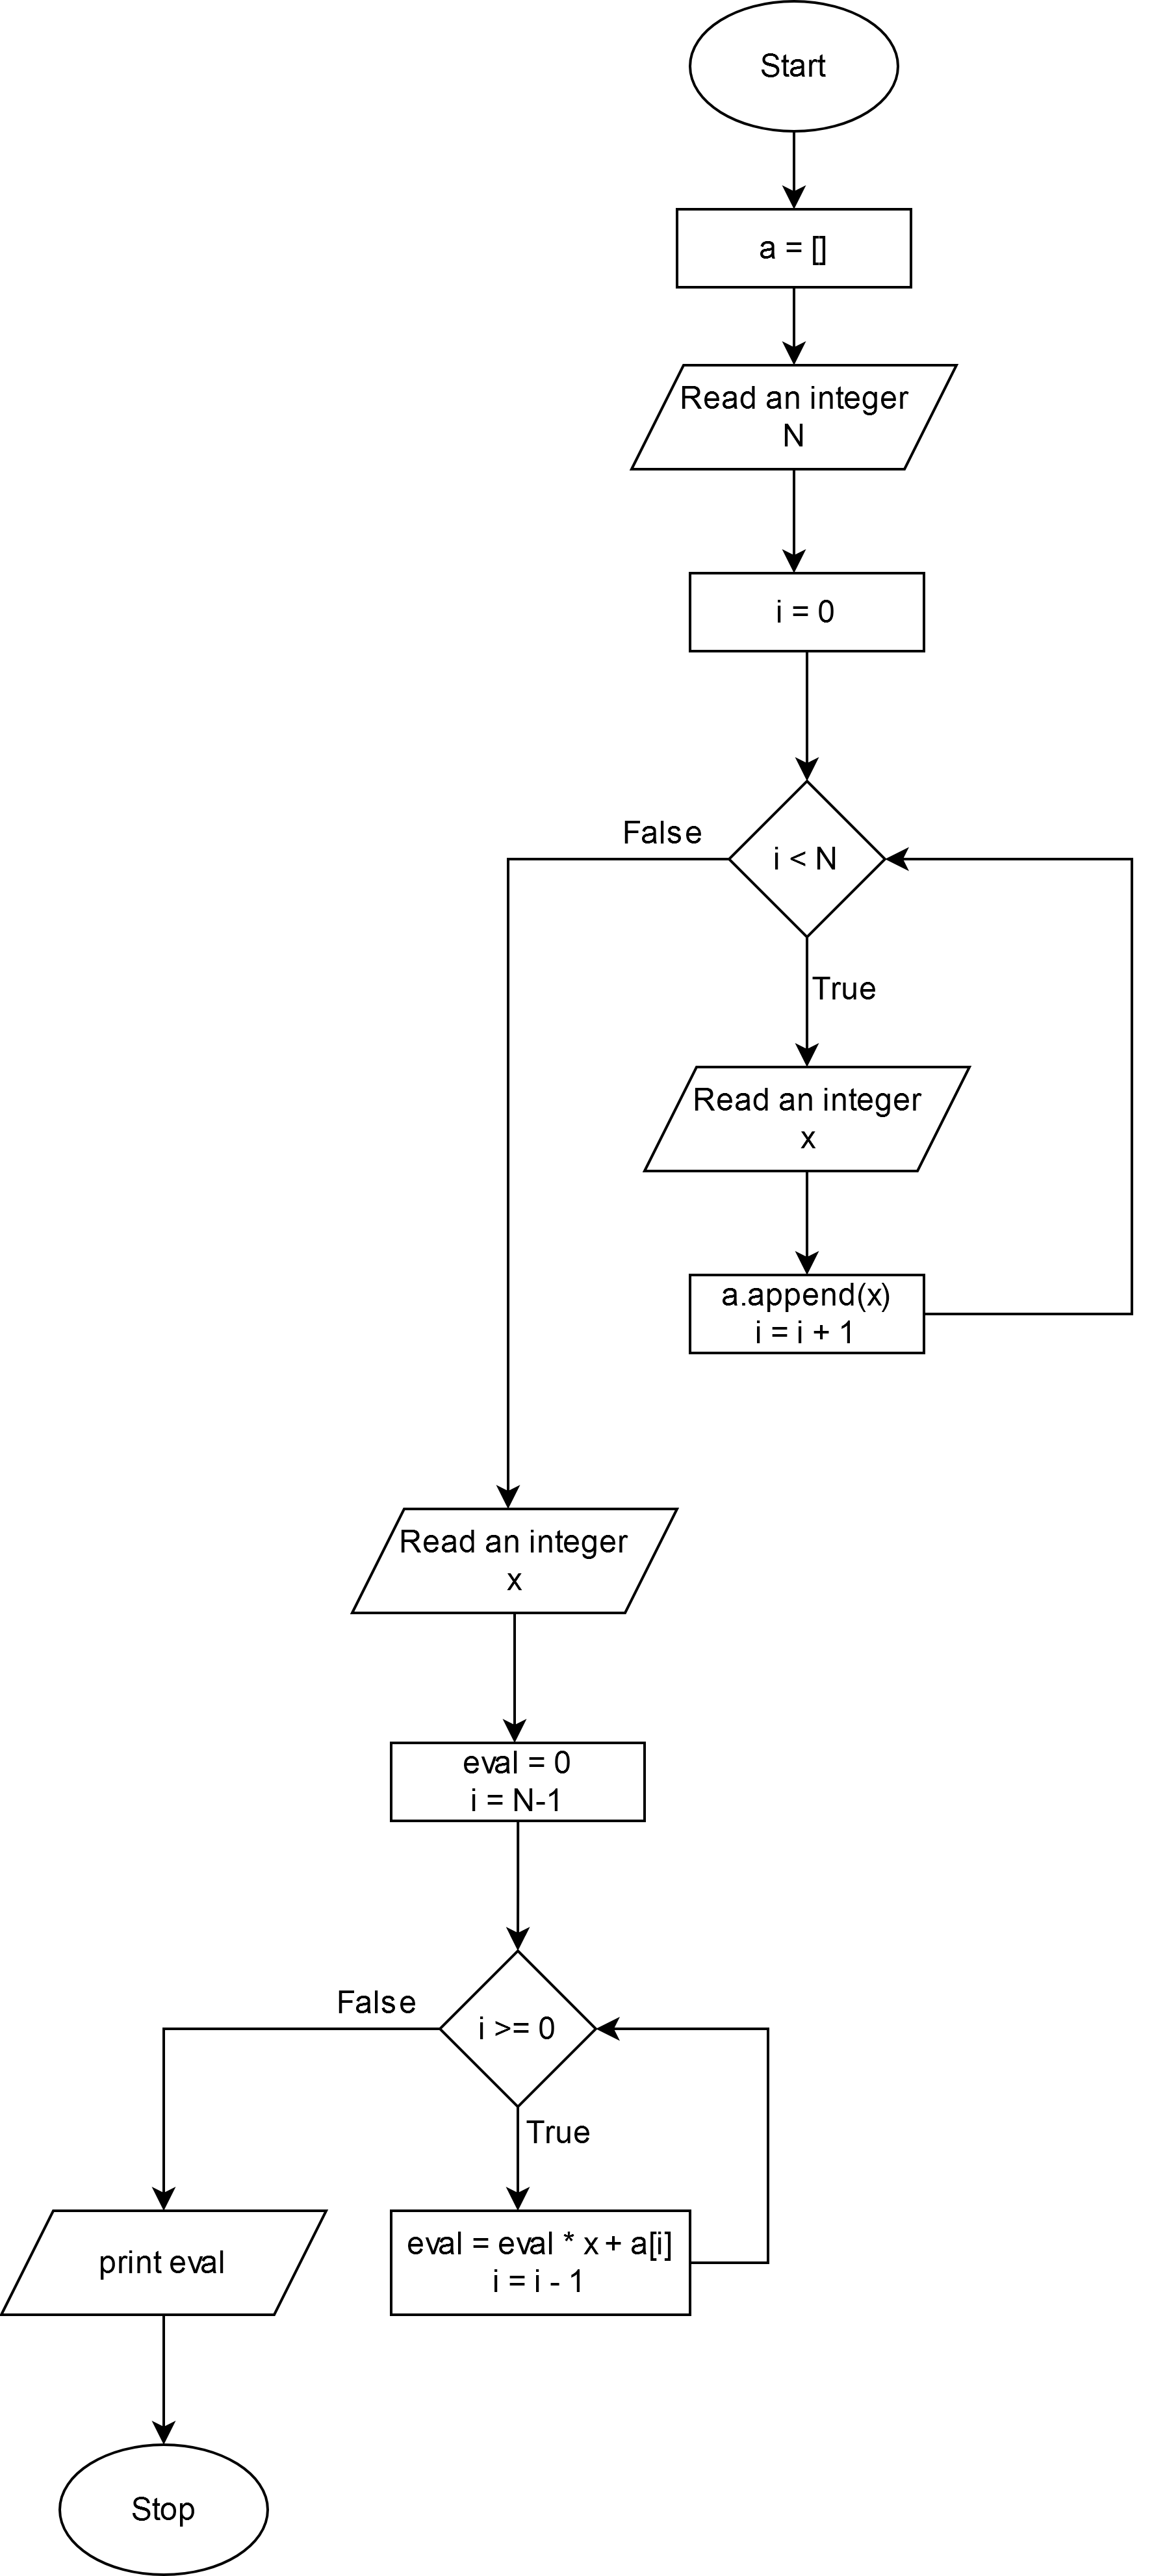
\includegraphics[width=0.5\textwidth]{Q6.png}
    \caption{Sample flowchart for Q6}
    \label{Q6}
\end{figure}

\clearpage

\begin{flushleft}

    \textbf{Q 7. } Draw a flowchart that takes as input the coefficients of a polynomial and 
    prints all the possible number of positive real zeros that it can have (in increasing order) 
    as predicted by Descartes’ rule of signs. 
    (Read the rule from the wikipedia page and implement it in the flowchart).

    Specifically the input should be 
    \begin{enumerate}
        \item A positive integer N, denoting the number of coefficients
        \item N integers denoting the coefficients. 
        If the numbers taken as input are \lstinline{P[0], P[1], ... P[n-1]}, 
        then the polynomial is $P[0] + P[1] x + P[2] x^2 + ... P[n-1] x^{n-1}$
    \end{enumerate}
    
    For example for the input
        4
        -1 -1 1 -1
    the output should be
        0 2
    because the polynomial is $-1 -x + x^2-x^3$,
    the number of changes in sign is 2, so the number of positive real roots can be either 0 or 2 according to the rule of signs, so the output should be 
        0 2
    \end{flushleft}
    
    \begin{flushleft}
    
    \textbf{Ans. } Note that coefficients that are $0$ must be ignored, that is if there are any 
    coefficients that are 0, then they must be ignored and the adjacent elements must be non-zero.
    Some corner cases are that the polynomials $-1-x^2, 1+x^2, -1-x^3, 1+x^3$ all have 0 changes in sign.
    The polynomial $1-x^3$ has 1 change in sign.

    One way to implement this is to maintain a variable \lstinline{last_sign} that stores the sign (1 if 
    positive and -1 if negative) of the last \textbf{non-zero} coefficient that is read.
    Initially the value of \lstinline{last_sign} should be 0.

    Then we should update \lstinline{last_sign} only when the current coefficient is not zero.

    This is shown in Fig \ref{Q7}.
    Once the number of sign changes is correctly identifies, we can iterate from \lstinline{sign_changes%2} 
    up to the number of sign changes, incrementing by 2 each time and printing the coefficients in that order.
    
    \end{flushleft}
    
    \begin{flushleft}
    
    \textbf{Grading. } Any flowchart that give the correct output for all valid inputs give 2, if there are any 
    errors in the flowchart but the logic is correct then 1.
    
    \end{flushleft}
    
    \begin{figure}[ht]
        \centering
        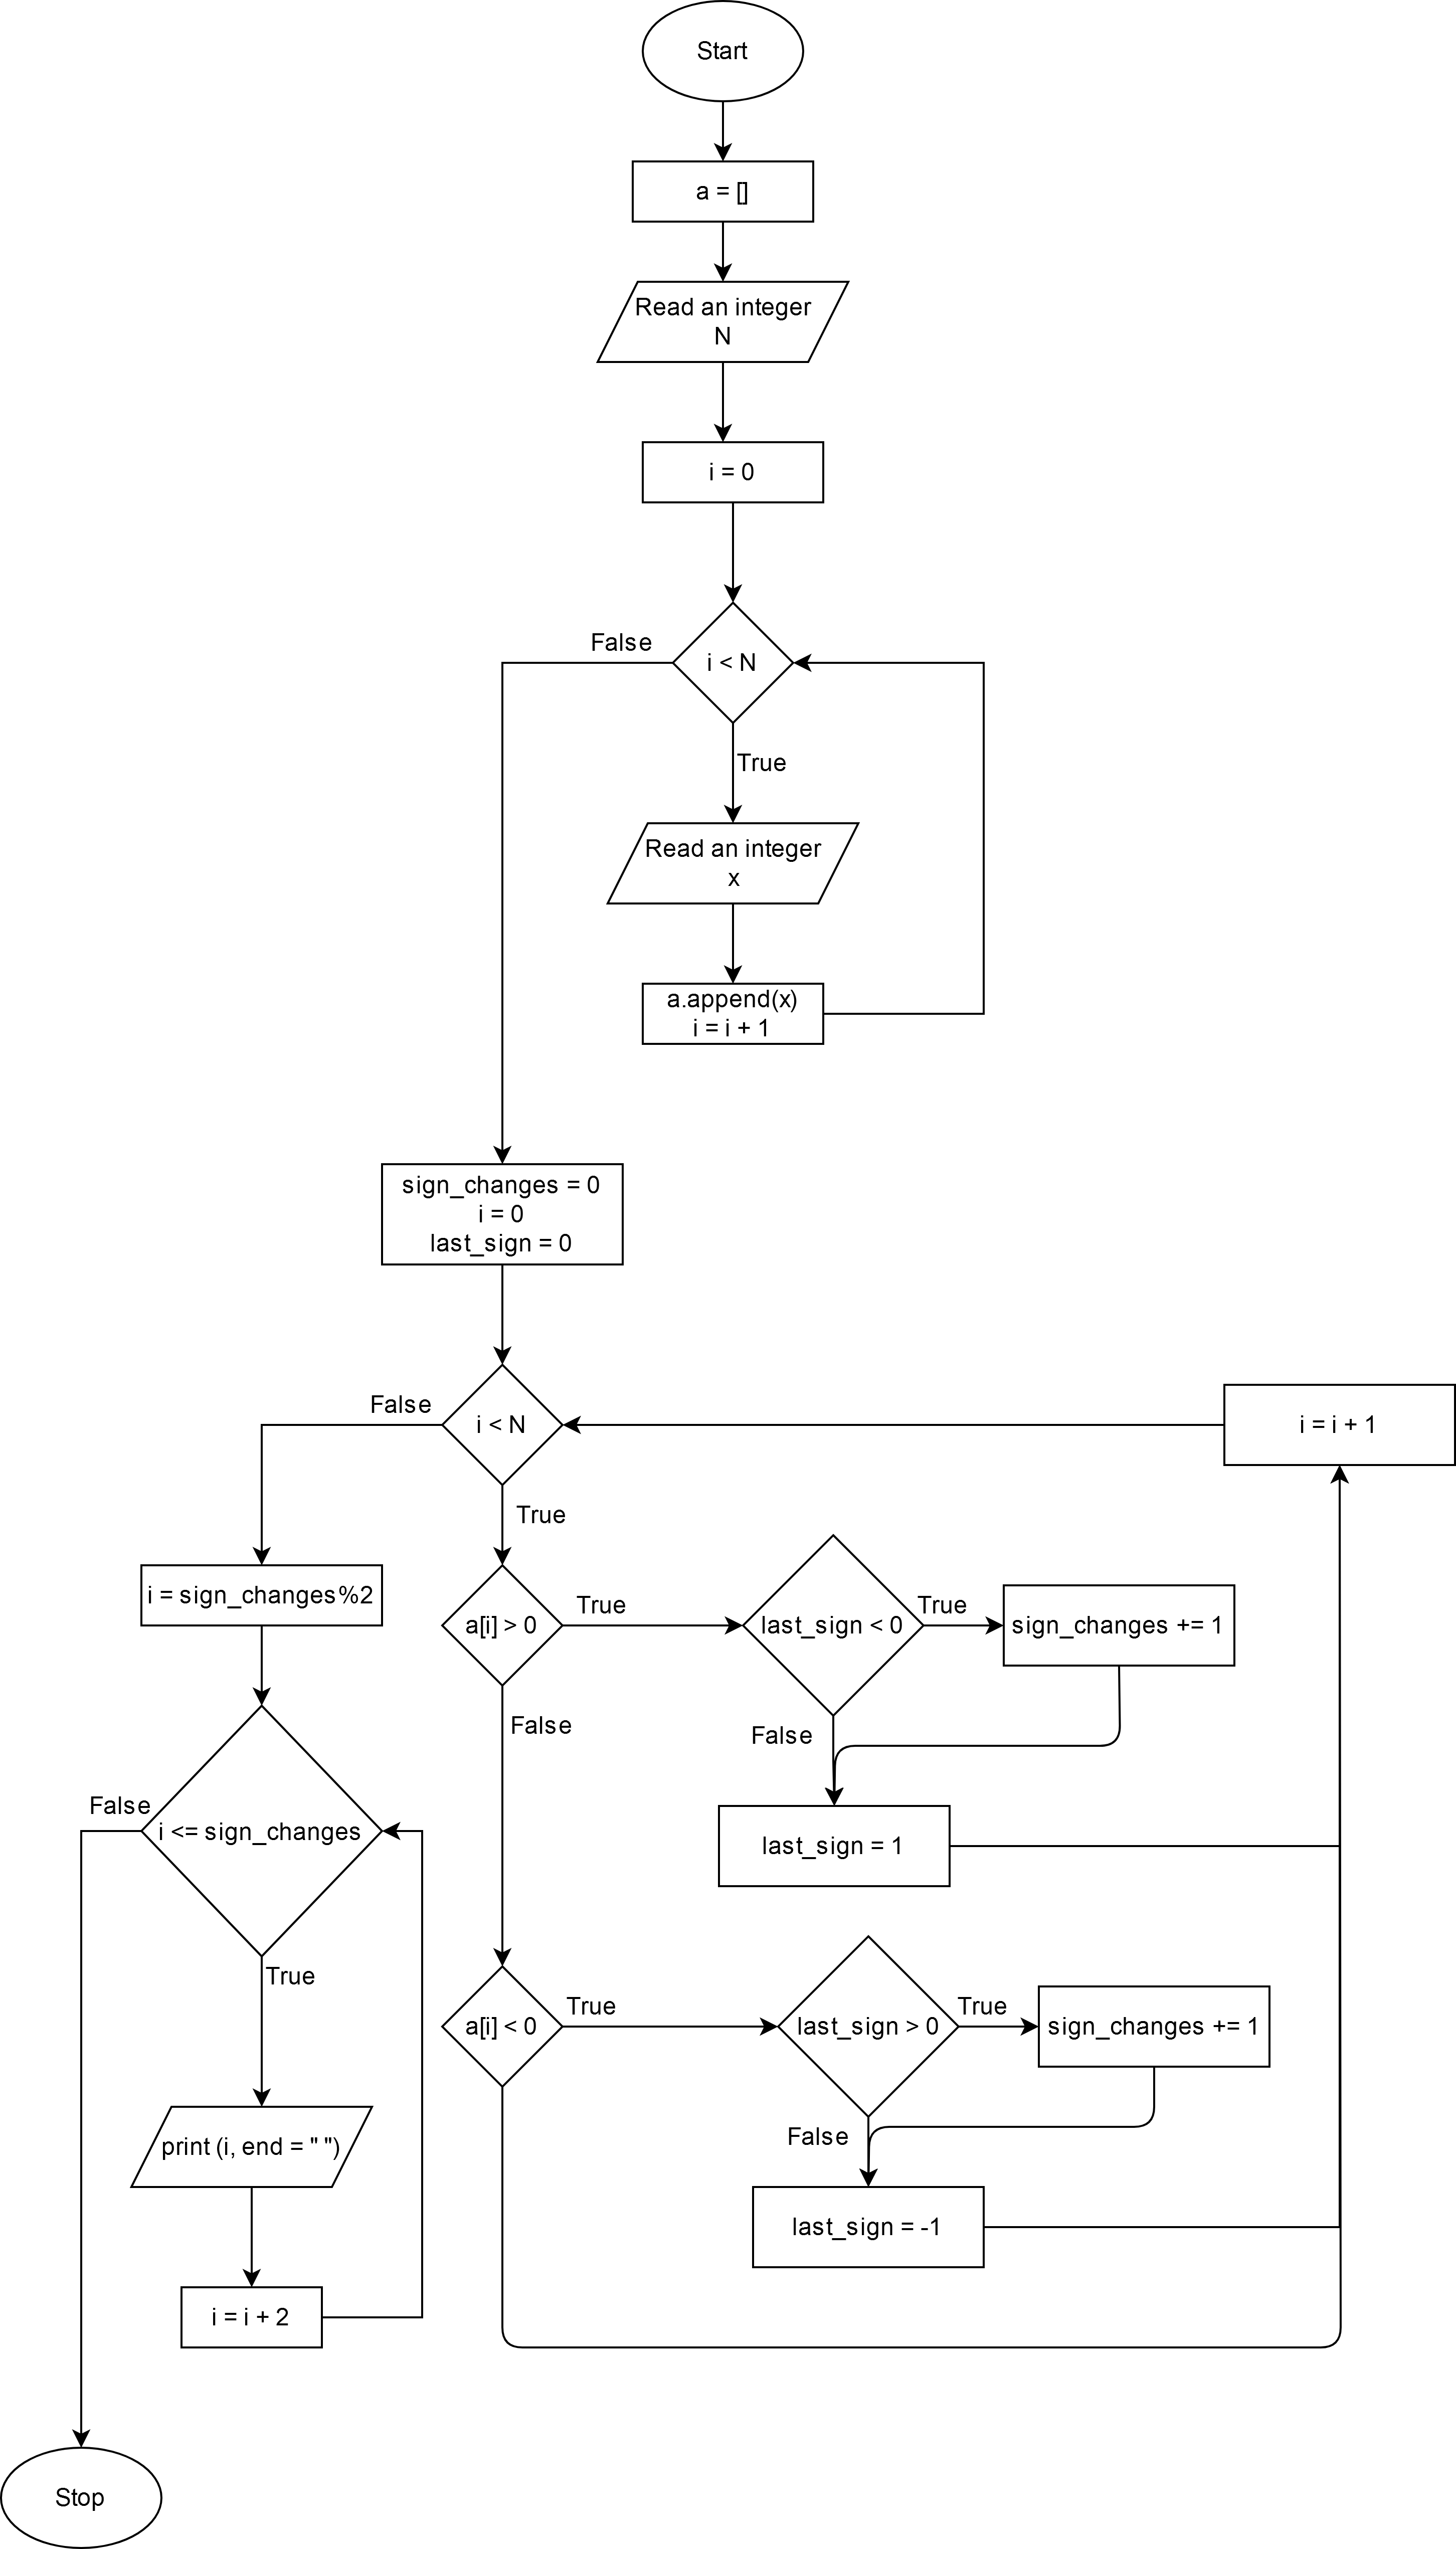
\includegraphics[width=0.5\textwidth]{Q7.png}
        \caption{Sample flowchart for Q7}
        \label{Q}
    \end{figure}
    
    \clearpage

\comment{

\begin{flushleft}

\textbf{Q 1. } 

\end{flushleft}

\begin{flushleft}

\textbf{Ans. } 

\end{flushleft}

\begin{flushleft}

\textbf{Grading. }

\end{flushleft}

\begin{figure}[ht]
    \centering
    \includegraphics[width=0.5\textwidth]{}
    \caption{Sample flowchart for Q}
    \label{Q}
\end{figure}

\clearpage
}

\end{document}